\documentclass[sigconf,screen,review]{acmart}
\settopmatter{printacmref=false}
\setcopyright{none}
\acmConference[WWW Companion '27]{Companion Proceedings of the ACM Web Conference 2027}{May 10--14, 2027}{Dublin, Ireland}
\usepackage{booktabs}
\usepackage{xcolor}
\usepackage{xspace}
% Every \pending{} must be resolved before submission (checked by `make check`).
\newcommand{\pending}[1]{\textcolor{red}{[PENDING: #1]}}
% Generated by src/make_numbers.py from results/. Do not edit by hand.
\newcommand{\authorAgree}{58 of 60 (97\%)\xspace}
\newcommand{\authorItems}{20\xspace}
\newcommand{\browserN}{1,463\xspace}
\newcommand{\browserTwice}{94\xspace}
\newcommand{\browserUnused}{118\xspace}
\newcommand{\bsCdF}{0.58\xspace}
\newcommand{\bsCdP}{0.85\xspace}
\newcommand{\bsCdPCI}{0.78--0.90\xspace}
\newcommand{\bsCdR}{0.44\xspace}
\newcommand{\bsDead}{82\xspace}
\newcommand{\bsN}{1,403\xspace}
\newcommand{\bsSampled}{114\xspace}
\newcommand{\bsSmF}{0.55\xspace}
\newcommand{\bsSmP}{0.43\xspace}
\newcommand{\bsSmPCI}{0.28--0.61\xspace}
\newcommand{\bsSmR}{0.77\xspace}
\newcommand{\bsUhF}{0.33\xspace}
\newcommand{\bsUhP}{0.54\xspace}
\newcommand{\bsUhPCI}{0.32--1.00\xspace}
\newcommand{\bsUhR}{0.24\xspace}
\newcommand{\calBlocked}{214\xspace}
\newcommand{\calBlockedReachable}{86\xspace}
\newcommand{\calBlockedStill}{97\xspace}
\newcommand{\calBlockedTried}{193\xspace}
\newcommand{\calFiltered}{34\xspace}
\newcommand{\calPlainAlive}{59.8\%\xspace}
\newcommand{\calRedirect}{186\xspace}
\newcommand{\calRedirectMoved}{126\xspace}
\newcommand{\changedBing}{3.7\%\xspace}
\newcommand{\changedClusterCI}{3.1--5.5\%\xspace}
\newcommand{\changedN}{60\xspace}
\newcommand{\changedNeeva}{5.4\%\xspace}
\newcommand{\changedPpl}{4.4\%\xspace}
\newcommand{\changedRate}{4.3\%\xspace}
\newcommand{\changedYou}{1.1\%\xspace}
\newcommand{\checkableBing}{374\xspace}
\newcommand{\checkableNeeva}{391\xspace}
\newcommand{\checkablePpl}{547\xspace}
\newcommand{\checkableYou}{91\xspace}
\newcommand{\ctlChangedExcess}{50\%\xspace}
\newcommand{\ctlChangedN}{36\xspace}
\newcommand{\ctlChangedNow}{58\%\xspace}
\newcommand{\ctlChangedThen}{8\%\xspace}
\newcommand{\ctlExcess}{12\%\xspace}
\newcommand{\ctlExcessCI}{3--24\%\xspace}
\newcommand{\ctlStillExcess}{10\%\xspace}
\newcommand{\ctlStillN}{29\xspace}
\newcommand{\ctlStillNow}{17\%\xspace}
\newcommand{\ctlStillThen}{7\%\xspace}
\newcommand{\eFourAgree}{93\%\xspace}
\newcommand{\eFourAgreeExNever}{89\%\xspace}
\newcommand{\eFourLinkAgree}{87\%\xspace}
\newcommand{\eFourN}{60\xspace}
\newcommand{\eFourPairs}{166\xspace}
\newcommand{\eFourTotal}{225\xspace}
\newcommand{\eFourUnmatched}{59\xspace}
\newcommand{\eOneCascBa}{0.77\xspace}
\newcommand{\eOneCoAuc}{0.86\xspace}
\newcommand{\eOneCoAucCI}{0.83--0.88\xspace}
\newcommand{\eOneCoBa}{0.78\xspace}
\newcommand{\eOneCoBaCI}{0.75--0.81\xspace}
\newcommand{\eOneCoFone}{0.67\xspace}
\newcommand{\eOneMcAuc}{0.82\xspace}
\newcommand{\eOneMcAucCI}{0.78--0.84\xspace}
\newcommand{\eOneMcBa}{0.75\xspace}
\newcommand{\eOneMcBaCI}{0.72--0.78\xspace}
\newcommand{\eOneMcFone}{0.63\xspace}
\newcommand{\eOneNgAuc}{0.78\xspace}
\newcommand{\eOneNgAucCI}{0.75--0.81\xspace}
\newcommand{\eOneNgBa}{0.73\xspace}
\newcommand{\eOneNgBaCI}{0.70--0.76\xspace}
\newcommand{\eOneNgFone}{0.59\xspace}
\newcommand{\eOneQwBa}{0.64\xspace}
\newcommand{\eOneQwBaCI}{0.61--0.67\xspace}
\newcommand{\eOneQwFone}{0.45\xspace}
\newcommand{\eOneQwSupRate}{85\%\xspace}
\newcommand{\eOneThr}{0.75\xspace}
\newcommand{\eThreeArchFail}{37 of the 73\xspace}
\newcommand{\eThreeArchFetch}{2\xspace}
\newcommand{\eThreeArchLookup}{35\xspace}
\newcommand{\eThreeExplainGpuGB}{9.1\xspace}
\newcommand{\eThreeGpuGB}{3.4\xspace}
\newcommand{\eThreeJudgeS}{1.5\xspace}
\newcommand{\eThreeMedianS}{92\xspace}
\newcommand{\eThreeN}{20\xspace}
\newcommand{\eThreeNetShare}{97\%\xspace}
\newcommand{\eThreePairs}{3\xspace}
\newcommand{\eThreeUrls}{2\xspace}
\newcommand{\estCI}{9--33\%\xspace}
\newcommand{\estNo}{5\%\xspace}
\newcommand{\estNotFull}{20\%\xspace}
\newcommand{\estStillNotFull}{17\%\xspace}
\newcommand{\evN}{1,232\xspace}
\newcommand{\evNone}{20.9\%\xspace}
\newcommand{\evPresent}{76.7\%\xspace}
\newcommand{\figItem}{dev-880\xspace}
\newcommand{\figPnow}{0.57\xspace}
\newcommand{\figPthen}{0.97\xspace}
\newcommand{\insAwayDifferent}{15 of 17 (88\%)\xspace}
\newcommand{\insAwayN}{18\xspace}
\newcommand{\insChangedEv}{22 of 36 (61\%)\xspace}
\newcommand{\insChangedN}{38\xspace}
\newcommand{\insChangedPrec}{22 of 37 (59\%)\xspace}
\newcommand{\insDemotedFull}{12 of 19 (63\%)\xspace}
\newcommand{\insDemotedN}{19\xspace}
\newcommand{\insOneChangedPrec}{21 of 43 (49\%)\xspace}
\newcommand{\insOneN}{100\xspace}
\newcommand{\insStillAgree}{24 of 29 (83\%)\xspace}
\newcommand{\insStillN}{29\xspace}
\newcommand{\insTwoN}{128\xspace}
\newcommand{\insUncertainN}{20\xspace}
\newcommand{\insUncertainNotFull}{8 of 20 (40\%)\xspace}
\newcommand{\jcChanged}{60\xspace}
\newcommand{\jcN}{1,038\xspace}
\newcommand{\jcRate}{5.8\%\xspace}
\newcommand{\judgeBothMs}{291\xspace}
\newcommand{\judgeMedianMs}{96\xspace}
\newcommand{\judgeMissEv}{115\xspace}
\newcommand{\linkBing}{9.1\%\xspace}
\newcommand{\linkLostCI}{8.8--12.0\%\xspace}
\newcommand{\linkLostClusterCI}{8.2--12.5\%\xspace}
\newcommand{\linkLostN}{144\xspace}
\newcommand{\linkLostRate}{10.3\%\xspace}
\newcommand{\linkNeeva}{10.5\%\xspace}
\newcommand{\linkPpl}{11.5\%\xspace}
\newcommand{\linkYou}{6.6\%\xspace}
\newcommand{\lostBing}{12.8\%\xspace}
\newcommand{\lostBingCI}{9.8--16.6\%\xspace}
\newcommand{\lostCI}{12.8--16.5\%\xspace}
\newcommand{\lostClusterCI}{12.2--16.9\%\xspace}
\newcommand{\lostN}{204\xspace}
\newcommand{\lostNeeva}{15.9\%\xspace}
\newcommand{\lostNeevaCI}{12.6--19.8\%\xspace}
\newcommand{\lostPpl}{15.9\%\xspace}
\newcommand{\lostPplCI}{13.1--19.2\%\xspace}
\newcommand{\lostRate}{14.5\%\xspace}
\newcommand{\lostUpperRate}{18.4\%\xspace}
\newcommand{\lostYou}{7.7\%\xspace}
\newcommand{\lostYouCI}{3.8--15.0\%\xspace}
\newcommand{\nCheckable}{1,403\xspace}
\newcommand{\nDev}{1,106\xspace}
\newcommand{\nPairs}{2,203\xspace}
\newcommand{\nStill}{1,145\xspace}
\newcommand{\nTest}{1,097\xspace}
\newcommand{\nThenSupported}{1,627\xspace}
\newcommand{\nUnverPairs}{224\xspace}
\newcommand{\nUrls}{1,473\xspace}
\newcommand{\qwenMedianS}{0.8\xspace}
\newcommand{\smCatchChanged}{50\xspace}
\newcommand{\smNoMatchStill}{363\xspace}
\newcommand{\smNoMatchStillPct}{31.7\%\xspace}
\newcommand{\subCoAuc}{0.79\xspace}
\newcommand{\subMcAuc}{0.78\xspace}
\newcommand{\subN}{627\xspace}
\newcommand{\subNgAuc}{0.65\xspace}
\newcommand{\subShare}{57\%\xspace}
\newcommand{\testChangedRate}{4.0\%\xspace}
\newcommand{\testLinkLostRate}{9.9\%\xspace}
\newcommand{\toolCheckable}{1,275\xspace}
\newcommand{\toolLostCI}{13.6--17.6\%\xspace}
\newcommand{\toolLostRate}{15.5\%\xspace}
\newcommand{\trAuc}{0.86\xspace}
\newcommand{\trChangedPrec}{29 of 44 (66\%)\xspace}
\newcommand{\trChangedRate}{3.4\%\xspace}
\newcommand{\trChangedSampled}{50\xspace}
\newcommand{\trCheckable}{5,611\xspace}
\newcommand{\trFetchGapH}{14\xspace}
\newcommand{\trLinkLostRate}{10.0\%\xspace}
\newcommand{\trPairs}{8,834\xspace}
\newcommand{\uhHalluLinkLost}{40\xspace}
\newcommand{\uhHalluStill}{7\xspace}
\newcommand{\uhLiveChanged}{57\xspace}
\newcommand{\uhLiveLinkLost}{60\xspace}
\newcommand{\uhLiveLinkLostPct}{42\%\xspace}
\newcommand{\uhLiveLost}{117\xspace}
\newcommand{\uhLiveLostPct}{57.4\%\xspace}
\newcommand{\uncertainN}{54\xspace}
\newcommand{\uncertainRate}{3.8\%\xspace}
\newcommand{\urlLost}{142\xspace}
\newcommand{\urlLostPct}{9.6\%\xspace}
\newcommand{\urlReachable}{1,105\xspace}
\newcommand{\urlReachablePct}{75.0\%\xspace}
\newcommand{\urlUnver}{226\xspace}
\newcommand{\urlUnverPct}{15.3\%\xspace}
\newcommand{\wbCapture}{41\xspace}
\newcommand{\wbFiltered}{8\xspace}
\newcommand{\wbN}{54\xspace}
\newcommand{\wbReachable}{8\xspace}


\begin{document}
\sloppy
\title{CiteDrift: Do the Pages Cited by AI Search Answers Still Support Them?}
\author{Seungbum Ju}
\affiliation{\institution{Samsung Electronics}\city{Seoul}\country{Republic of Korea}}
\email{seungbum.ju@samsung.com}

\begin{abstract}
AI search engines back their statements with links, and readers keep those answers long after they were generated. A citation that supported a statement when it was made can later stop doing so, either because the link dies or because the page is rewritten. Link checkers see only the first case, and claim verifiers applied to a live citation see only the page as it is today. We demonstrate CiteDrift, a system that checks every statement--citation pair of an answer twice, against the page as it was when cited and as it is today, and reports whether support persisted, was lost with the link, or was lost through a change of content. CiteDrift runs entirely on one consumer GPU with open models. Re-checking \nPairs pairs from four generative search engines (2023) in October 2026, we find that \linkLostRate (95\% CI \linkLostClusterCI) of the checkable citations that annotators had judged fully supporting lost their link, a link-only checker reports \uhLiveLinkLostPct of these lost links as live, and CiteDrift flags a further \changedRate as content changes; an AI agent blind to our outcomes confirmed \insChangedPrec of a sample of these flags. The demo offers an explorer of these results and a local mode that checks any pasted answer.

\end{abstract}
\keywords{AI search, citation verification, reference rot, web evolution, claim verification}
\maketitle

\section{Introduction}
Generative search engines answer a query with a few sentences and attach URLs to them. The links make an answer look checkable, and answers are kept and reused: they are shared as links, pasted into reports and stored in chat histories. Whether the cited page supports a statement, however, is a property of the page \emph{at a given time}. The Web changes underneath citations: in scholarly articles, ``one in five articles suffers from reference rot''~\cite{Klein_2014} and ``three out of four URI references lead to changed content''~\cite{Jones_2016}. For AI search answers, verifiability has been measured once, at generation time, by human annotators~\cite{Liu_2023} or by automatic auditors~\cite{Wu_2025,venkit2025deeptraceauditingdeepresearch}.

Existing tools cover the two halves of the problem separately. Link checkers such as urlhealth~\cite{rao2026detectingcorrectingreferencehallucinations} decide whether a cited URL resolves, but a page that still loads can have stopped saying what the answer claims. Claim verifiers and attribution evaluators~\cite{Tang_2024,Gao_2023,Yue_2023} judge a statement against the document they are given; applied to a live citation, that is the page as it is today, so they cannot tell a citation that never supported a statement from one that did and then changed.

CiteDrift joins the two. For each statement--citation pair it judges support on the page as cited (an archived capture, or the page text saved with a dataset) and on the page today, and assigns one of six outcomes: \emph{still supported}, \emph{content changed}, \emph{uncertain}, \emph{link lost}, \emph{could not check}, or \emph{not supported when cited}. The contributions are:
(1) a two-time, claim-level citation checker with a calibrated link-state step that separates bot walls and network filters from real loss and judges redirects by content;
(2) a fully local implementation (no commercial API; one 12\,GB GPU) with a web explorer and a check mode for any answer; and
(3) a measurement: re-checking the human-annotated development and test citations of Liu et al.~\cite{Liu_2023} after about three and a half years, \linkLostRate of the checkable citations judged fully supporting in 2023 lost their link (a link-only checker reports \uhLiveLinkLostPct of these as live), and CiteDrift flags another \changedRate as content changes.
The demo relates to the Responsible Web track (information integrity, auditing), Search and Retrieval-Augmented AI (evaluation of AI search), and Web Mining (Web evolution).

\section{System}
\label{sec:system}
\begin{figure*}[t]
\centering
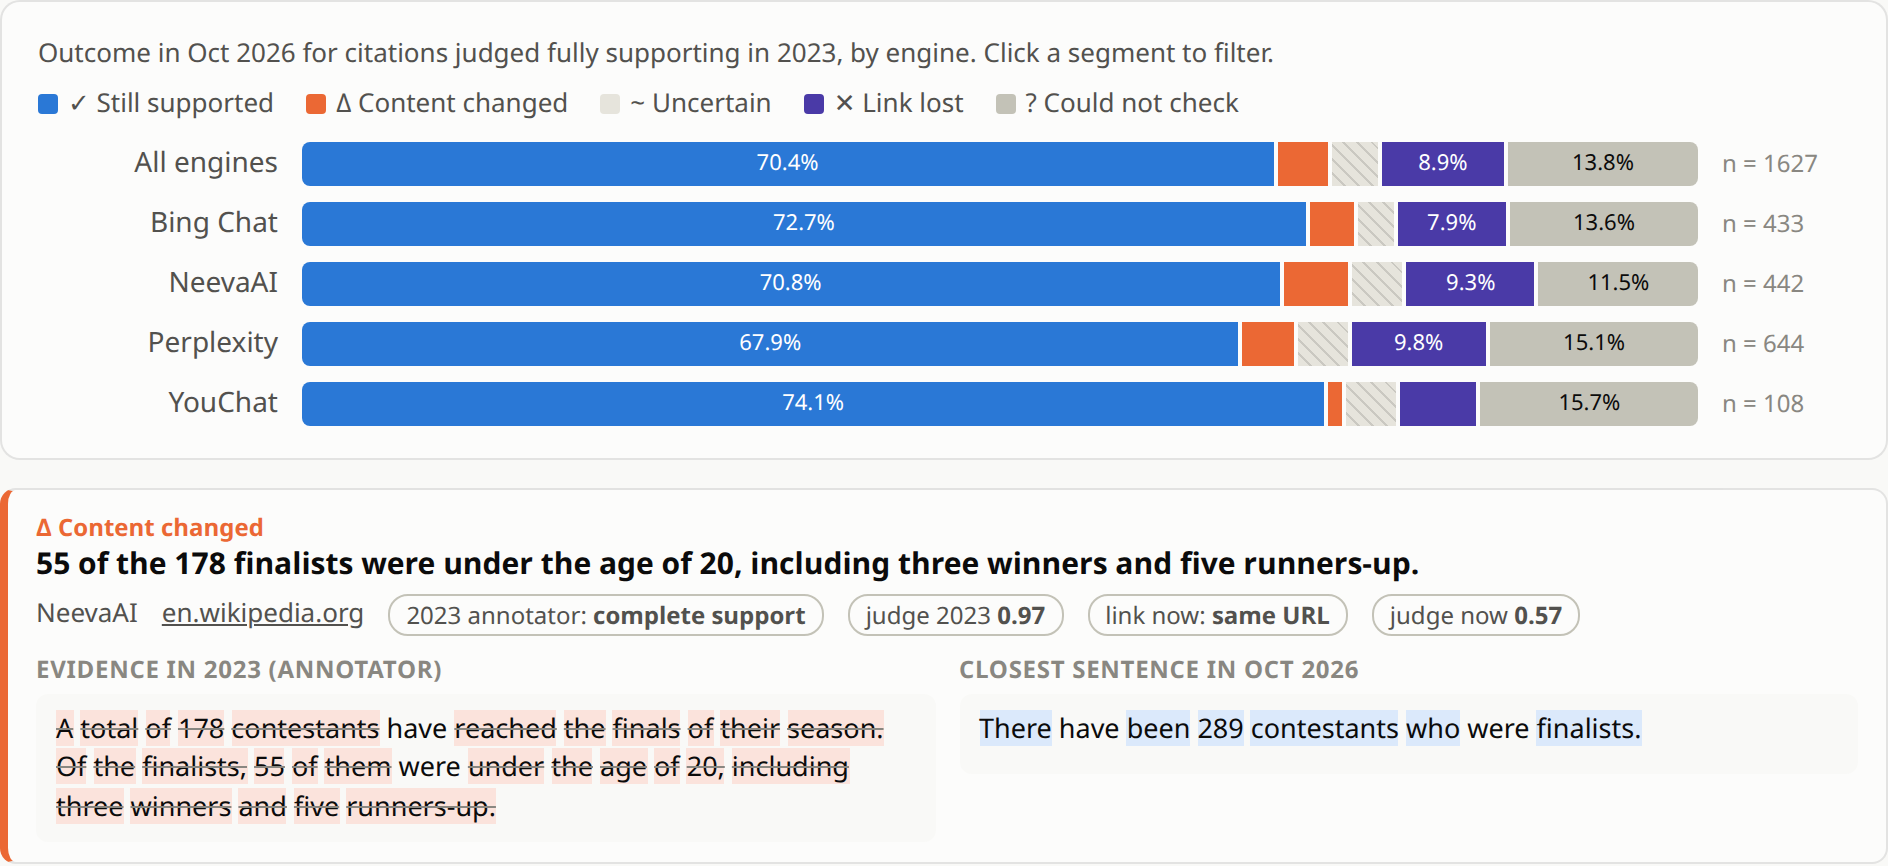
\includegraphics[width=0.77\textwidth]{figures/ui_explorer.png}
\caption{CiteDrift explorer. Top: outcome in October 2026 of all citations that annotators judged fully supporting in 2023, including those that could not be checked, per engine (segments filter the list). Bottom: one pair; the 2023 evidence and today's closest sentence are aligned word by word: the page is still online, some figures changed, and the judge's score dropped from \figPthen to \figPnow.}
\label{fig:ui}
\end{figure*}
CiteDrift takes an answer with citation markers (\texttt{[1]}, \texttt{[2]}, \dots), the list of cited URLs and, optionally, the date of the answer. It splits the answer into sentences, pairs every sentence with the citations it carries, and processes each statement--citation pair in four steps (Fig.~\ref{fig:ui}).

\textbf{1. Link state.} Each URL is requested once by an identified client with per-host spacing. A plain HTTP request is not enough to decide that a link is lost: in our measurement, \calBlockedReachable{} of the \calBlockedTried{} URLs that answered a plain request with 401/403/429 and were re-opened opened normally in an ordinary browser, and \calFiltered{} URLs were answered by our own network's web filter rather than by the site. CiteDrift therefore (i) recognises filter and bot-wall pages by their text, (ii) re-opens refused pages in an ordinary desktop browser (in the batch measurement for every refused page not answered by our network filter; on request in check mode); it does not solve challenges or bypass paywalls, and a page that appears only after a detected bot interstitial counts as a bot wall, and (iii) judges redirects by content, not by URL: a redirect counts as \emph{moved} if the new page still contains at least 30\% of the cited page's word 5-grams or keeps its title (thresholds set before the evaluation from pages that kept their URL and redirects to a site root; script in the repository), and as \emph{redirected elsewhere} otherwise; without a ``then'' page only redirects to a site root count as lost. With this rule \calRedirectMoved{} of \calRedirect{} redirects were moves. The resulting states fall into three groups: \emph{reachable} (same URL, moved), \emph{lost} (dead, error page, redirected elsewhere) and \emph{unverifiable} (bot wall, network filter, server or TLS error, time-out, empty page, not requested).

\textbf{2. Then and now text.} The ``now'' page is reduced to its main content with Trafilatura~\cite{Barbaresi_2021}; the full visible DOM text is judged as well and the higher score counts, so that an extraction miss is not mistaken for a content change. The ``then'' page is the Internet Archive capture closest to the answer date, or page text saved with a dataset when available (for Liu et al., text extracted by the dataset authors' HTML-to-text pipeline). Archive lookups that fail (e.g., HTTP~429) are reported as such and never read as ``the page did not exist''.

\textbf{3. Support judge.} MiniCheck-Flan-T5-Large~\cite{Tang_2024} (our re-implementation of its reference inference) scores the statement against every $\sim$500-word chunk of a page and keeps the best chunk. Because AI search answers often copy phrases from their sources, the MiniCheck logit is combined with the share of the statement's word 4-grams found on the page (logistic regression fitted on the development split). The decision threshold is fixed on the development split and used unchanged at both time points.

\textbf{4. Outcome.} A pair is \emph{not supported when cited} if the judge rejects the ``then'' page, \emph{link lost} or \emph{could not check} according to its link state, and \emph{still supported} if the judge accepts today's page. Because the judge errs, a rejection today alone is not called a change: a pair is \emph{content changed} only if, in addition, the passage that supported the statement then is no longer on today's page; if it is still there the pair stays still supported, and if the signals cannot be compared it is \emph{uncertain}. For flagged pairs, an optional explainer (Qwen2.5-7B-Instruct~\cite{qwen2025qwen25technicalreport}, 4-bit) reads the best passage and writes a one-sentence reason.

\textbf{Interface.} A single web application (FastAPI back end, plain HTML/JS front end) has two modes. The \emph{explorer} is a static page with our precomputed results on the Liu et al. data: per-engine outcome bars that act as filters, and one card per pair showing the statement, the annotator's 2023 evidence next to the closest sentence on today's page with a word-level diff, link state and both judge scores. The \emph{check} mode runs the full pipeline on a pasted answer on the user's own machine and streams each outcome as soon as its page has been fetched and judged; nothing the user submits leaves the machine except requests for the cited pages, their robots.txt files and their archive records.

\section{Evaluation}
\label{sec:eval}
\textbf{Data.} Liu et al.~\cite{Liu_2023} collected answers of Bing Chat, NeevaAI, Perplexity and YouChat between late February and late March 2023 and had annotators judge each statement--citation pair (complete, partial or no support), copying evidence sentences from the page. The release also contains the text of each cited page, released with the dataset (extracted with DOM Distiller and Trafilatura); we use it as the ``then'' page. We develop and report on the development (\nDev pairs) and test (\nTest) splits, \nPairs pairs and \nUrls distinct URLs re-fetched on 15 October 2026, and keep the training split (\trPairs pairs) as an untouched held-out check, re-fetched about \trFetchGapH hours later. After calibration, \urlReachable URLs (\urlReachablePct) were reachable, \urlLost (\urlLostPct) lost and \urlUnver (\urlUnverPct) could not be checked from our network.

\textbf{E1: judge accuracy.} Table~\ref{tab:e1} compares judges on the 2023 text against the annotators' labels (target: complete support; threshold chosen on dev, reported on test). MiniCheck alone and word 4-gram overlap are close on average because these engines often copy phrases from their sources, but on the \subShare of test statements that share few 4-grams with the page, MiniCheck (AUC \subMcAuc) is far better than string matching (\subNgAuc). Their combination is best overall. Qwen2.5-7B (4-bit) on the three best chunks accepts \eOneQwSupRate of all pairs and is weaker as a verifier; we use it only to explain flags.

\begin{table}[t]
\caption{E1: support judges on the 2023 page text vs.\ the annotators' labels (test split, $n=$\nTest; 95\% bootstrap CIs).}
\label{tab:e1}
\small
\begin{tabular*}{\columnwidth}{@{\extracolsep{\fill}}lccc@{}}
\toprule
Judge & AUC & Bal.\ acc. & F1$_\text{unsup.}$\\
\midrule
Word 4-gram overlap & \eOneNgAuc & \eOneNgBa & \eOneNgFone\\
MiniCheck-Flan-T5-L & \eOneMcAuc & \eOneMcBa & \eOneMcFone\\
Qwen2.5-7B (4-bit), top-3 chunks & -- & \eOneQwBa & \eOneQwFone\\
\textbf{MiniCheck + overlap (ours)} & \textbf{\eOneCoAuc} & \textbf{\eOneCoBa} & \textbf{\eOneCoFone}\\
\quad 95\% CI & \eOneCoAucCI & \eOneCoBaCI & \\
\bottomrule
\end{tabular*}
\end{table}

\textbf{E2: drift 2023$\rightarrow$2026.} We take the \nThenSupported pairs that annotators judged \emph{fully} supporting; \nUnverPairs of them could not be checked, leaving \nCheckable. With the annotators' evidence available, a reachable pair that the judge rejects today counts as \emph{content changed} only if the judge accepted the 2023 text \emph{and} not all of the annotator's evidence is still on today's page; if all of it is still there it stays still supported (\judgeMissEv pairs), otherwise it is \emph{uncertain}. \linkLostN citations (\linkLostRate; 95\% CI \linkLostClusterCI, bootstrap over URLs) lost the link, \changedN (\changedRate, CI \changedClusterCI) are flagged as content changes, and \uncertainN (\uncertainRate) are uncertain (Table~\ref{tab:e2}). On the test split alone, which played no part in fitting the judge (the outcome rule was chosen on a spot-check sample that included test pairs), the rates are \testLinkLostRate and \testChangedRate. On the held-out training split, processed the same way after all design choices were fixed, the judge reaches AUC \trAuc on the 2023 text, \trLinkLostRate of \trCheckable checkable citations lost the link and \trChangedRate are flagged as content changes; a fresh blind AI agent confirmed \trChangedPrec of the decidable flags in a sample of \trChangedSampled.

\begin{table}[t]
\caption{E2: outcome in Oct 2026 of citations judged fully supporting in 2023 (share of checkable pairs), and how well each method finds lost support (estimated over all \bsN checkable pairs: spot-check sample weighted by stratum, the \bsDead pairs on dead or error pages counted as lost).}
\label{tab:e2}
\small
\begin{tabular*}{\columnwidth}{@{\extracolsep{\fill}}lrrr@{}}
\toprule
Engine & checkable & link lost & content changed\\
\midrule
Bing Chat & \checkableBing & \linkBing & \changedBing\\
NeevaAI & \checkableNeeva & \linkNeeva & \changedNeeva\\
Perplexity & \checkablePpl & \linkPpl & \changedPpl\\
YouChat & \checkableYou & \linkYou & \changedYou\\
\midrule
Method & precision & recall & F1\\
urlhealth (not LIVE) & \bsUhP & \bsUhR & \bsUhF\\
String match (4-gram) & \bsSmP & \bsSmR & \bsSmF\\
\textbf{CiteDrift} & \textbf{\bsCdP} & \bsCdR & \bsCdF\\
\bottomrule
\end{tabular*}
\end{table}

\textbf{Validation.} We have no human labels for 2026, so AI agents (Claude, a fresh context for each sample), blind to all methods and shown each statement, the annotator's evidence, both URLs and the page text, labelled stratified random samples. On the first (\insOneN items), only \insOneChangedPrec content changes flagged by a looser rule (either signal alone) were confirmed, so we adopted the two-signal rule; we report the second, fresh sample (\insTwoN items). There the agent confirmed \insChangedPrec flagged content changes as no longer fully supported, \insAwayDifferent ``redirected elsewhere'' links as leading to a different document, and \insStillAgree ``still supported'' pairs. Because the agents and the 2023 annotators can simply disagree, another agent labelled the same pairs on the \emph{2023} text: it already judged \ctlStillThen of the still-supported pairs and \ctlChangedThen of the flagged changes not fully supported in 2023 (vs.\ \ctlStillNow and \ctlChangedNow today; \ctlStillN and \ctlChangedN pairs labelled both times). The flagged changes are thus mostly real changes rather than labeller disagreement. Netting out the disagreement and weighting by stratum size, content changes remove full support from about \ctlExcess (CI \ctlExcessCI) of the reachable citations, possibly more than CiteDrift flags; it rests mostly on the few sampled still-supported pairs judged changed. The two-signal rule trades recall for precision. The author re-checked \authorItems of the second sample's items by hand and agreed with \authorAgree of the agent's labels.

\textbf{Baselines.} urlhealth~\cite{rao2026detectingcorrectingreferencehallucinations} reports \uhLiveLinkLost of the \linkLostN lost links as live, nearly all of them redirects to a home page or another document, and calls \uhHalluStill still-supported citations ``likely hallucinated''. It labelled \wbN URLs ``likely hallucinated'' although annotators read all of them in 2023; \wbReachable of them load normally for CiteDrift, \wbFiltered were answered by our network filter, a later re-query found archive records for \wbCapture, and its code turns any failed archive lookup into ``no snapshot''. Over all checkable citations (Table~\ref{tab:e2}), urlhealth misses most lost support. String matching on today's page (same text views as CiteDrift) finds the most, but more than half of its flags are false (precision \bsSmP), likely because answers paraphrase; CiteDrift is the conservative option (precision \bsCdP, CI \bsCdPCI), at the cost of recall; the two F1 scores do not differ reliably, and the reference (the agent's 2026 label) includes labeller disagreement, which lowers every method's recall.

\textbf{E3--E4: cost and check mode.} On one RTX~5070 (12\,GB), judging one statement against both views of today's page takes a median \judgeBothMs\,ms. Checking a whole answer (\eThreeN test answers; median \eThreeUrls URLs, archive capture as ``then'') takes a median \eThreeMedianS\,s, of which \eThreeNetShare is spent waiting on polite page and archive requests and \eThreeJudgeS\,s on judging; peak GPU memory is \eThreeGpuGB\,GB (\eThreeExplainGpuGB\,GB with the explainer, measured on five answers). For \eThreeArchFail statement--citation pairs no archived ``then'' page could be retrieved (\eThreeArchLookup lookup errors, mostly without a logged cause, and \eThreeArchFetch refused capture fetches); such pairs are marked as having no ``then'' page, and on reachable pages they are labelled still supported if today's page supports them and uncertain otherwise. Run on \eFourN test answers with the dataset's 2023 text, check mode, run without its optional browser re-check, agreed with the E2 tool-mode outcome on \eFourAgree of the \eFourPairs pairs it could match to E2 (of \eFourTotal; \eFourAgreeExNever without pairs both judged unsupported in 2023); most differences are pages that the batch run had opened in a browser.

\textbf{Limitations.} The ``then'' text was extracted differently from today's; outcomes depend on one network vantage point and fetch time; \nUnverPairs supported citations could not be checked; and the 2026 validation rests on an AI labeller. Outcomes are therefore shown with scores and evidence for the reader to inspect.

\section{Demonstration}
\label{sec:demo}
At the venue we bring a machine with one consumer GPU (all measurements here are on a 12\,GB desktop RTX~5070) running the full system: the explorer works offline, check mode needs the venue network. Visitors can (1) browse the 2023$\rightarrow$2026 explorer, click an engine's ``content changed'' segment and read, side by side, the sentence an annotator copied in 2023 and what the page says today, or list the \uhLiveLost citations that lost support although urlhealth reports their link as live; (2) paste an answer they obtained from any AI search engine during the conference, optionally with a past date, and see each citation's outcome appear, with both judge scores and the passages that decided it, as its page is fetched; and (3) toggle the explainer to see why a citation was flagged. Visitors without a GPU can replay recorded checks of five 2023 answers in the public explorer. The code is at \url{https://github.com/seungbum/citedrift}, the public explorer at \url{https://seungbum.github.io/citedrift/}, and a two-minute video walk-through at \url{https://seungbum.github.io/citedrift/citedrift_demo.mp4}.

\section{Related Work}
\label{sec:related}
\textbf{Reference rot.} Studies of scholarly articles separate link rot from content drift and find both common~\cite{Klein_2014,Jones_2016}; CiteDrift measures both for AI search citations, per statement rather than per URL.
\textbf{Citation and attribution checking.} Liu et al.~\cite{Liu_2023} audited four generative search engines with annotators; SourceCheckup~\cite{Wu_2025} and DeepTRACE~\cite{venkit2025deeptraceauditingdeepresearch} automate such audits with LLM judges; ALCE~\cite{Gao_2023} and AttrScore~\cite{Yue_2023} evaluate attribution automatically; Facts\&Evidence~\cite{Boonsanong_2025} checks claims against multiple evidence sources. All judge support at one point in time.
\textbf{Link checking and freshness.} urlhealth~\cite{rao2026detectingcorrectingreferencehallucinations} classifies cited URLs as live, stale or likely hallucinated using the Wayback Machine, without looking at content. OwlerLite~\cite{Zerhoudi_2026} detects page changes to keep a retrieval index fresh before answering; CiteDrift audits citations after an answer was given.

\section{Ethical Use of Data}
\label{sec:ethics}
We use only public data, the verifiability judgments of Liu et al.~\cite{Liu_2023} (MIT licence); no human participants were involved, and the 2026 spot checks were labelled by AI agents on locally stored text. Requests to cited sites: (i) our identified client, once per URL for the measurement (at least five seconds between requests to a host), and once per run for the pages of the \eThreeN E3 answers (three full runs; explainer runs on one and twice on five answers), the \eFourN E4 answers (four runs) and example answers citing six sites (about twenty test and video runs, plus a few pilot and connectivity tests), two seconds apart per host (a host's robots.txt and first page request were unspaced until a late fix); sites that ask automated clients not to fetch a page were never requested (redirect targets were not re-checked); (ii) one visit with an ordinary browser under automation for \browserN refused, failing or empty pages (\browserTwice twice; \browserUnused dead training-split pages opened under a broader rule are not used), without solving challenges, logging in or bypassing paywalls; pages reached only after a detected bot interstitial count as bot walls; (iii) one urlhealth check per fetchable development/test URL, run as published (HEAD, a GET after some errors, an archive lookup after a 404; browser user agent), rate-limited like all our archive lookups. Page bodies stay local: the public explorer shows the dataset's evidence and at most one current-page sentence (up to 300 characters) per pair. Check mode processes the answer locally, stores nothing, and requests only the cited pages, their robots.txt files and archive records (and, on request, one browser visit; one such test was run).


\begin{acks}
\textbf{Generative AI disclosure.} We used a generative AI assistant (Anthropic Claude) to implement the system and the experiment scripts, run the experiments, produce the 2026 validation labels (as stated in Section~\ref{sec:eval}), collect bibliographic metadata, and draft the text. The author defined the problem formulation and venue scope, directed key design decisions (including the two-signal drift threshold), independently conducted the author hand-check on the validation sample (Section~\ref{sec:eval}), interpreted the empirical findings, and reviewed and revised the manuscript, taking full responsibility for all content and conclusions.

\end{acks}

\bibliographystyle{ACM-Reference-Format}
\bibliography{refs}
\end{document}
